\documentclass[10pt]{article}


\usepackage{arxiv}

\usepackage[utf8]{inputenc} % allow utf-8 input
\usepackage[T1]{fontenc}    % use 8-bit T1 fonts
\usepackage{hyperref}       % hyperlinks
\usepackage{url}            % simple URL typesetting
\usepackage{booktabs}       % professional-quality tables
\usepackage{amsfonts}       % blackboard math symbols
\usepackage{amsmath}        % for \DeclareMathOperator
\usepackage{bm}             % bold math
\usepackage{nicefrac}       % compact symbols for 1/2, etc.
\usepackage{microtype}      % microtypography
\usepackage{graphicx}       % Required for including images
\usepackage{booktabs}       % Top and bottom rules for tables
\usepackage{lipsum}

\newcommand{\real}{\mathbb{R}}
\newcommand{\nat}{\mathbb{N}}
\newcommand{\relu}{\mathrm{relu}}
\newcommand{\der}{\mathrm{d}}
\newcommand{\soft}{\mathrm{softmax}}
\newcommand{\kldiv}{\mathcal{D}_{KL}}
\newcommand{\bernoulli}{\mathrm{Bernoulli}}
\newcommand{\poisson}{\mathrm{Poisson}}
\newcommand{\E}{\mathrm{E}}
\DeclareMathOperator*{\argmax}{arg\,max}
\DeclareMathOperator*{\argmin}{arg\,min}

\title{Generative Outliers Detector Network}


\author{
  Jonathan Guymont \\
  Montréal Institute of Learning Algorithms\\
  Universite de Montréal\\
  Montréal, Canada\\
  \texttt{j.guymont@gmail.com}\\
}

\begin{document}
\maketitle

\begin{abstract}
	Spam detection is commonly used for email and text message filtering. We propose an unsupervised method to learn the distribution of text data using a generative model and propose a method to classify spam based on the learned distribution. Our experiment shows that this method can achieve good precision, making it useful for either 1) speeding up the labeling process of a data set or 2) labeling a certain percentage of the data in order to switch to a semi-supervised learning method or 3) iteratively removing the detected spams from the data and and retraining the model to relearn the distribution of the non-spam more efficiently, since there would be less spam in the data.
\end{abstract}

\keywords{Generative model \and Unsupervised classification \and NLP}

\section{Introduction}
\label{sec:intro}
A standard approach for detecting spams is to use a dataset with labeled spam and non-spam examples. Then a classifier can be trained to discriminate between spam and non-spam messages. This approach requires a lot of time to label the data, thus it would be interesting to see how an unsupervised method would perform since unsupervised methods do not require labeled data. We propose to use a generative model to learn the distribution of a dataset assumed to be \emph{highly} unbalanced, where the underrepresented class is the spam. If we suppose that the spam and the non-spam text are coming from 2 significantly distinct data generating processes, a model that is trained to learn the distribution of the entire data should mostly learn the distribution of the overrepresented class (here the non-spam).

We used a variational autoencoder \cite{kingma2013auto} to learn the distribution of the data. Variational Autoencoders are generative models that can be seen as a two parts neural network: an encoder network $Q(z|x)$ that encode the most relevant information of the features into a latent variable $z$, and a decoder network $P(x|z)$ that reconstructs the distribution of the inputs from the latent variable $z$. After the model is trained, the decoder network should be good at generating data that comes from the same distribution as the training set. Thus, if our training data mostly contains non-spam messages, it should be good at reconstructing non-spam examples, but not so good at reconstructing spam. So if $x$ is a spam, its reconstruction density $P(x|z)$ should be low and we should classify it as spam. More formally, we find a threshold $\mathcal{T}$ such that when the density of an example is lower then $\mathcal{T}$, the example is classified as spam. We propose a simple method for determining $\mathcal{T}$ in section \ref{subsection:oultiers}.

The following section contains theoretical background on VAE and can be skipped by the reader who is familiar with the subject. Section 3 describes an approach for unsupervised spam detection. Section 4 provides experimental results on the SMS Spam Collection Data Set\footnote{https://archive.ics.uci.edu/ml/datasets/sms+spam+collection} along with details on the experiment. Section 5 contains a discussion including a concluding remark.

\section{Theoretical Background}
\paragraph{Latent variable models} Variational autoencoders are generative models. Generative models are models that learn the underlying distribution of the data, e.g. $p(\mathbf{x})$ when the task is density estimation or $p(\mathbf{x}, \mathbf{y})$ in supervised classification. It is possible to express the prior $p(\mathbf{x})$ as a function of a latent variable model $\mathbf{z}$
\begin{equation}
	p(\mathbf{x}) 
	= \int p_\theta (\mathbf{x}|\mathbf{z}) p(\mathbf{z}) \der\mathbf{z}
\end{equation}
This modelization allows us to generate samples from $p(\mathbf{x})$ by first sampling $\mathbf{z}$ from $p(\mathbf{z})$ and then sampling $\mathbf{x}$ from $p_\theta(\mathbf{x}|\mathbf{z})$. Since the latent space is large, it would be impossible to learn a good representation for $p_\theta(\mathbf{x}|\mathbf{z})$ without a good mapping $f\colon \mathcal{Z}\times \Theta \mapsto \mathcal{X}$, where $\mathcal{Z}$ is the latent space, $\theta\in\Theta$, and $\mathcal{X}$ is the input space. In other words, we need pairs $(\mathbf{z}, \mathbf{x})$ such that $\mathbf{x}$ is likely to be generated by $\mathbf{z}$ in order to find a good parametrization for the posterior of $\mathbf{x}$. It is also possible to modelize the prior of the latent as function of the data $\mathbf{x}$
\begin{equation}
	p(\mathbf{z}) 
	= \int p(\mathbf{z}|\mathbf{x}) p(\mathbf{x}) \der\mathbf{x}
\end{equation}
During training, instead of sampling $\mathbf{z}$ from its prior, we can sample $\mathbf{z}$ by first sampling $\mathbf{x}$ from $p(\mathbf{x})$ and then sample $\mathbf{z}$ from $p(\mathbf{z}|\mathbf{x})$. Since $p(\mathbf{x})$ is unknown, we sample uniformly from the training set $D_n$ instead. Also, the posterior of the latent variable $p(\mathbf{z}|\mathbf{x})$ is intractable, so we use an approximation $q_\phi(\mathbf{z}|\mathbf{x})$. Finally, we can approximate the prior of the data by sampling $\mathbf{z}^{(1)}$,...,$\mathbf{z}^{(L)}$ from $q_\phi(\mathbf{z}|\mathbf{x})$ and then using $p(\mathbf{x})= \int p_\theta (\mathbf{x}|\mathbf{z}) p(\mathbf{z}) \der\mathbf{z}\approx \frac{1}{L}\sum_{i=1}^L p_\theta(\mathbf{x}|\mathbf{z}^{(i)})$.

\paragraph{Variational lower bound} During training, both $p_\theta(\mathbf{x}|\mathbf{z})$ and $q_\phi(\mathbf{z}|\mathbf{x})$ are trained simultaneously $-$ the objective being the maximization of the marginal likelihood of the prior of the data $\log p(\mathbf{x})$. Let's consider the Kullback-Leibler divergence $\kldiv$ between $p(z|x)$ and $q(z|x)$
\begin{equation}
	\begin{split}
	\kldiv[q(z|x)||p(z|x)] 
	=& \E_{z\sim q(z|x)}[ \log q(z|x) - \log p(z|x)]\\
	=& \E_{z\sim q(z|x)}[ \log q(z|x) - \log p(x|z) - \log p(z) + \log p(x)]\\
	=& \log p(x) + \E_{z\sim q(z|x)}[ \log q(z|x)  - \log p(z)] - \E_{z\sim q(z|x)}\log p(x|z)\\
	=& \log p(x) - \kldiv[q(z|x)||p(z|x)] - \E_{z\sim q(z|x)}\log p(x|z)\\
	\end{split}
\end{equation}
If we move all the terms on the right except the marginal likelihood to the left we have
\begin{equation}
	\begin{split}
	\log p(x) = 
	\E_{z\sim q(z|x)}\log p(x|z)- \kldiv[q(z|x)||p(z)] + \kldiv[q(z|x)||\log p(z|x)]\\
	\end{split}
\end{equation}
The term $\kldiv[q(z|x)||\log p(z|x)]$ is intractable, but because of Gibbs' inequality, we know that it is positive and thus we have
\[
\log p(x)  \geq \E_{z\sim q(z|x)}\log p(x|z)- \kldiv[q(z|x)||p(z)]
\]
Hence, our loss function is
\[
\mathcal{L} = \E_{z\sim q(z|x)}\log p(x|z)- \kldiv[q(z|x)||p(z)]
\]
If we set the distribution of the latent variable to be a multivariate standard Gaussian, i.e. $\mathbf{z}\sim \mathcal{N}(\bm{0}, \mathbf{I})$, we can express the KL-divergence between $q(z|x)$ and $p(z)$ as
\begin{equation}
	\kldiv[q(z|x)||p(z)] 
	= \frac{1}{2}\sum_{j=1}^J \mu_j^2 + \sigma_j^2 - 1 - \log \sigma_j^2
\end{equation} 
where $J$ is the dimension of the latent variable (see \cite{kingma2013auto} for details). Thus the loss function that we want to minimize is
\begin{equation}
	\mathcal{L} 
	= -\E_{z\sim q(z|x)}\log p(x|z) + \frac{1}{2}\sum_{j=1}^J \mu_j^2 + \sigma_j^2 - 1 - \log \sigma_j^2
\end{equation}

\section{Method}
\subsection{Density estimation}
We tried 3 different approaches to represent the distribution of the text messages. The first model aims to learn the distribution of the binarized representation of the bag of words (BOW), i.e. each feature is either one or zero depending on whether the word corresponding to the position of the features is present in the sentence or not. The second one is to learn the distribution of the standard BOW representation. The last model learns the distribution of the \emph{bag of characters} in the text message. In this section, we describe the general form of the encoder and the different decoders used in each of these models. All models have 2 neural networks: an encoder network $f(\mathbf{x};\phi)$ that outputs the parameters of the posterior distribution of the latent variable and a decoder network $g(\mathbf{z};\theta)$ that outputs the parameters of the posterior distribution of the input. For all models, the latent variable is a standard Gaussian with a diagonal covariance. A neural network $f(\cdot)$ outputs the mean and the variance of the posterior latent distribution, i.e. we have $\bm{\mu}_z,\log\bm{\sigma}_z^2 = f(\mathbf{x};\phi)$ with $q_\phi(\mathbf{z}|\mathbf{x}) = \mathcal{N}(\mathbf{z};\bm{\mu}_z, \bm{\sigma}_z^2)$. In the simplest case, $f(\mathbf{x};\phi)$ is a one layer MLP
\begin{equation}
	\begin{split}
		\mathbf{h} =& \relu\left(\mathbf{W}_{xh}\mathbf{x}+\mathbf{b}_{xh}\right)\\
		\bm{\mu}_z =& \mathbf{W}^{(1)}_{hz}\mathbf{h}+\mathbf{b}^{(1)}_{hz}\\
		\log \bm{\sigma}_z^2 =& \mathbf{W}^{(2)}_{hz}\mathbf{h}+\mathbf{b}^{(2)}_{hz}\\
		\phi =& \{\mathbf{W}^{(1)}_{hz}, \mathbf{b}^{(1)}_{hz}, \mathbf{W}^{(2)}_{hz}, \mathbf{b}^{(2)}_{hz}, \mathbf{W}_{xh}, \mathbf{b}_{xh}\}
	\end{split}
\end{equation}
We can sample the latent variable using $\mathbf{z}=\bm{\mu}_z + \bm{\sigma}_z\odot \bm{\epsilon}$ where $\bm{\epsilon}\sim \mathcal{N}(\bm{0}, \bm{I})$. When experimenting, we change the form of the encoder by increasing the number of layers used to encode the last hidden layer $\mathbf{h}$ from which the parameters of the latent are read. Now we describe the structure of the different decoders we experimented with.
\paragraph{Bernoulli decoder} The first approach is to model the distribution of the binarized bag of words representation of the text messages. Let $\mathcal{V}$ be the size of the vocabulary of the training set and $\mathbf{x}\in \{0, 1\}^{|\mathcal{V}|}$ be the binarized bag of words representation of a text message. In this case, $\bm{\gamma}(\mathbf{z}) = g(\mathbf{z};\theta)$ and
\begin{equation}
	\log p_\theta(\mathbf{x}|\mathbf{z}) 
	= \sum_{i=1}^{|\mathcal{V}|}x_i\log\gamma_i(\mathbf{z}) + (1-x_i)\log(1-\gamma_i(\mathbf{z}))
\end{equation}
where $\gamma_i(\mathbf{z})$ can be seen as the parameter of $x_i \sim \bernoulli(x;\gamma_i(\mathbf{z}))$.

\paragraph{Poisson decoder} Our second approach is to model the distribution of the (non-binarized) BOW representation of the text messages. Let $\mathcal{V}$ be the vocabulary of the training set and $\mathbf{x}\in \nat^{|\mathcal{V}|}$ be the bag of words representation of a text message. Let $\bm{\lambda}(\mathbf{z})=g(\mathbf{z};\theta)$ be the output of the Poisson decoder network, i.e. the parameters of the posterior of the data. In this scheme, the probability that the word $i$ occur $x_i$ time is given by 
\begin{equation}
\poisson(x_i;\lambda_i(\mathbf{z}))
=e^{-\lambda_i(\mathbf{z})}\frac{\lambda_i^{x_i}(\mathbf{z})}{x_i!}
\end{equation}
Thus the log-likelihood is given by 
\begin{equation}
\log p_\theta(\mathbf{x}|\mathbf{z}) 
= \sum_{i=1}^{|\mathcal{V}|}x_i\log\lambda_i(\mathbf{z}) - \lambda_i(\mathbf{z}) -\log(x_i!)
\end{equation}
where $\log(x_i!)$ can be approximate by the Stirling approximation $\log(x_i!) \approx x_i \log x_i - x_i + \frac{1}{2} \log(2 \pi x_i)$. 
When fitting the character distribution, the only difference is that $\mathbf{x}\in \nat^{\mathcal{|C|}}$ where $\mathcal{C}$ is the set of characters in the training corpus. Note that even so the posterior distribution in both decoders assumes independence between the features, the prior distribution does not make this assumption since all the parameters are read from the same latent variable. In other words, the features $x_i$ and $x_j$, for $i$ different than $j$, are conditionally independent given the latent variable $\mathbf{z}$, but they are not independent.

\subsection{Outliers detection}
\label{subsection:oultiers}
A simple approach is to use the $k$-percentile of the learned distribution. When the model is trained, we evaluate the density of each example $p(\bm{x}^{(1)}),...,p(\bm{x}^{(n)})$ using $p(\mathbf{x})\approx\frac{1}{L}\sum_{i=1}^L p_\theta(\mathbf{x}|\mathbf{z}^{(i)})$, where $\mathbf{z}^{(i)}$ is sampled from the posterior distribution of the latent variable. Let $\tau$ be the index of the example such that $|\{\bm{x} : p(\bm{x}) < p(\bm{x}^{(\tau)})\}|=kn$ where $k\in (0, 1)$ should be smaller then the suspected percentage of spam in the data. Then the threshold is set to $\mathcal{T}=p(\bm{x}^{(\tau)})$.

\section{Experiment}

\subsection{Data}
For our experiment, we used the SMS Spam Collection Data Set containing spam
and non-spam labeled text messages (labels will be used only for testing the performance of
our model). Table \ref{tab:data} shows some examples of the text messages in the data. We selected 10\% of all the spam and all the non-spam examples. We split the data in two: 50\% of the data was used to develop the approach and 50\% was used to test it.

\begin{table}
	\caption{Sample data}
	\centering
	\begin{tabular}{ll}
		\toprule
		label     & text \\
		\midrule
		ham & Tell them the drug dealer's getting impatient \\
		ham & Oh... Lk tt den we take e one tt ends at cine lor... Dun wan yogasana oso can... \\
		spam & SIX chances to win CASH! From 100 to 20000 pounds txt CSH11 and send to 87575.\\
		spam & PRIVATE! Your 2003 Account Statement for 07808247860 shows 800 un-redeemed S.I.M. points. Call...\\
		\bottomrule
	\end{tabular}
	\label{tab:data}
\end{table}

\subsection{Preprocessing}
First note that the preprocessing was applied for both BOW models, but not for the \textit{bag of characters}. All punctuation was removed except for exclamation marks and question marks. We used regular expressions to replace email address and URL by \texttt{<email>} and \texttt{<URL>} respectively. The regular expressions were not catching every pattern so not all email and URL were replaced. We also tried to lemmatize the words, but as you can see in table \ref{tab:data} the spelling was often bad making it difficult to lemmatize the text. One option would be to use a spell checker, but we decide not to use any since some expressions may not be used as often in spam than in non-spam message or the other way around. For example, it is frequent to see \textit{u} instead of \textit{you} in non-spam texts; maybe this does not happen frequently in the spam text so by correcting this spelling error we may be removing a good feature.

\subsection{Architecture and training details}
For all models, both the encoder and the decoder were parametrized with 2 fully connected layers of 128 hidden units each. Relu activation function was applied to each hidden layer. We also applied dropout and batch normalization after each hidden layer. The dropout rate was set to 0.5. The output activation function of the Bernoulli decoder is the element wise sigmoid. For the Poisson decoder, the parameter of the posterior is given by 
\begin{equation}
	\bm{\lambda}(\mathbf{z}) = \exp(\bm{\alpha} \odot \tanh(\mathbf{o}_{\text{decoder}}))
\end{equation}
where $\mathbf{o}_{\text{decoder}}$ is the pre-activation output of the decoder and $\bm{\alpha}$ is a parameter that is read from the latent variable. Specifically,
\begin{equation}
	\begin{split}
	\eta =& \mathbf{W}_{z\alpha}\mathbf{z}+\mathbf{b}_{z\alpha}\\
	\bm{\alpha} =& 
		\begin{cases}
		0, \eta < 0,\\
		\eta, 0<\eta<3\\
		3, \eta > 3 
		\end{cases}
	\end{split}
\end{equation}
 The role of the parameter $\bm{\alpha}$ is to control the range of value of $\bm{\lambda}$. For the Bernoulli decoder, applying sigmoid at the end of the network is sufficient because the parameter of a Bernoulli is between 0 and 1. In the case of the Poisson distribution, $\lambda_i(\mathbf{z})$ is the expected value of the feature $x_i$ given $\mathbf{z}$. Thus, it is not as straight forward as in the Bernoulli case to control the range of possible values since $\bm{\lambda}$ is not upper bounded. The size of the latent variable is set to 20. We optimize all models parameters using \emph{Adam} \cite{2014arXiv1412.6980K} with a learning rate chosen among the set $[0.00003, 0.0001, 0.001]$, $\beta_1\in [0.5, 0.9]$ and $\beta_2 \in [0.99, 0.999]$. We used a batch size of 64 and optimize the model for 1000 iterations. The hyperparameters were selected so that the loss on the training set was minimized. When predicting whether an example was a spam or not, the threshold was set to the density corresponding to the $2.5\%$-percentile.

\subsection{Results}
Figure \ref{fig:result} and table \ref{table:result} summarize the result of the experiment. We used precision and recall as our evaluation metrics because the number of spams being significantly lower than the number of non-spams, the model could achieve 90\% by only predicting non-spam, making the accuracy a not very interesting metric. The precision is defined as the number of true spam detected over the total number of examples classified as spam including the misclassified one. The recall is defined as the number of true spam detected over the total number of spams in the data. We were mostly interested in achieving a good score on the precision since this would allow to remove the real spam of the data and iterate.
\begin{figure}[h]
	\centering
	\begin{tabular}{cccc}
		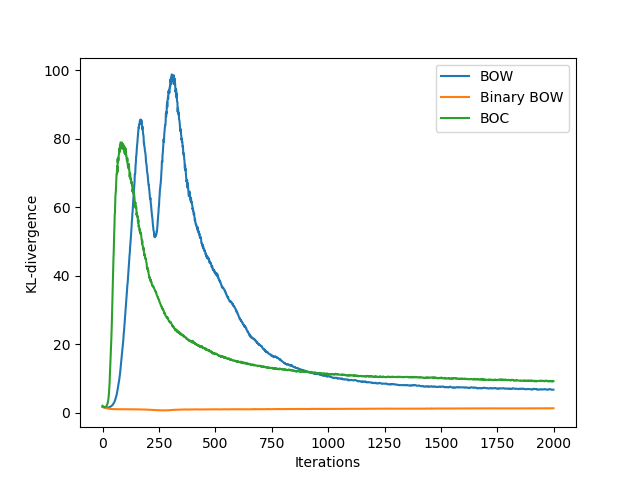
\includegraphics[width=0.4\textwidth]{../figures/kldiv_03.png}
		& 
		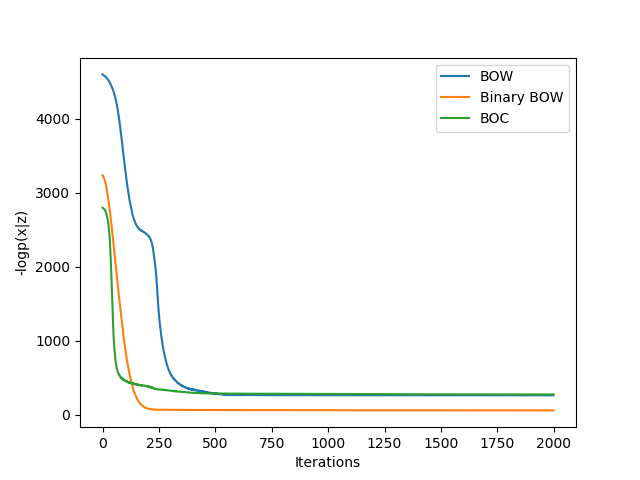
\includegraphics[width=0.4\textwidth]{../figures/logp_03.png}\\
		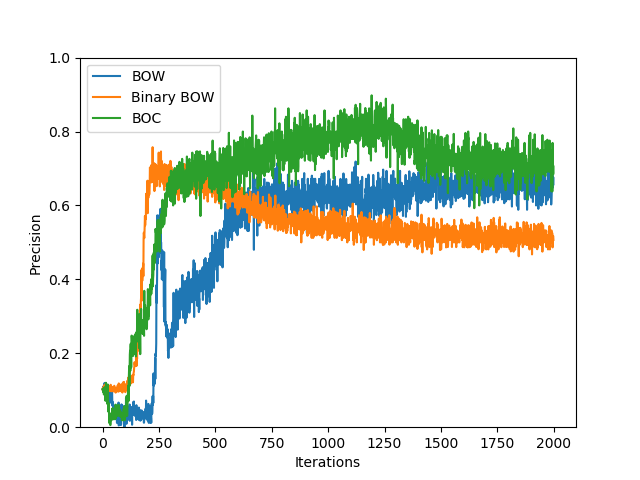
\includegraphics[width=0.4\textwidth]{../figures/precisions_03.png}
		& 
		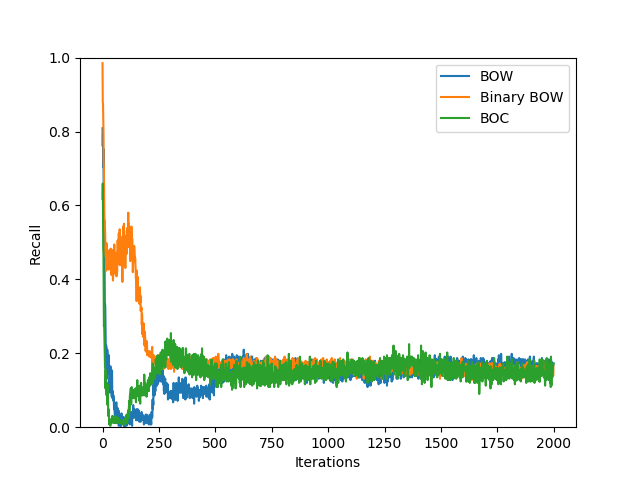
\includegraphics[width=0.4\textwidth]{../figures/recall_03.png}\\
	\end{tabular}
	\caption{\textbf{Top left.} KL-divergence over all training iterations for the 3 models. \textbf{Top right.} Negative log-likelihood over all training iterations for the 3 models. \textbf{Bottom left.} Precision of the model defined as the number of true spams detected over the total number of examples classified as spam including the misclassified one. \textbf{Bottom right.} Recall of the model defined as the number of true spams detected over the total number of spams in the data.}
	\label{fig:result}
\end{figure}
\begin{table}[h]
	\caption{Test results of the spam detection and the modelization of the text distribution. The test data represents 50\% of the entire data set. The confidence interval are due to the randomness caused by the sampling of the latent variable $\mathbf{z}$ when evaluating the probability.}
	\centering
	\begin{tabular}{lrrrr}
		\toprule
		model & precision & recall & $\log p(\mathbf{x}|\mathbf{z})$ & $\kldiv$\\
		\midrule
		BOW & $0.62\pm 0.006$ & $0.16\pm 0.004$ & $-258.62\pm 0.33$ & $8.27\pm 2.580$\\
		Binary BOW & $0.64\pm 0.003$ & $0.22\pm 0.003$ & $-48.89\pm 0.03$ & $1.25\pm 0.000$\\
		BOC & $0.79\pm0.005$ & $0.26\pm 0.004$ & $-279.95\pm 0.41$ & $14.17\pm 4.560$ \\
		\bottomrule
	\end{tabular}
	\label{table:result}
\end{table}
Note that there are confidence intervals on the results in table \ref{tab:result} due to the randomness caused by the sampling of the latent variable $\mathbf{z}$ when evaluating the probabilities. We can see in the top plots of figure \ref{fig:result} that the Bernoulli distribution (binary BOW model) was easier to learn then the Poisson's since both its KL-divergence and its log-likelihood converge to zero very fast. We suspect it is due to the simplicity of the Bernoulli distribution. Also, the precision of the Bernoulli model reach is maximum very fast. The recall seems to stabilize around 0.2 which is close to the percentile threshold of 0.25 that we used. The best precision on the spam detection task was achieved by the bag of characters model. This may be due to the large number of features of the BOW (4588) model when compared to the number of training examples (2671), especially since a large number of features were the same but because of the different spelling they had different representations.

\section{Discussion  and  conclusion}
The proposed method for spam detection could potentially be used for any anomaly detection related task. In particular, it is interesting to see that the character level distribution yields the best performance since it does not require preprocessing. Text preprocessing in often language-specific making language models that rely heavily on feature engineering hard to scale across different languages. Since the character level model does not require feature design, it would be interesting to see if it scales across languages. We note that it would be necessary to investigate how sensitive the results are to the choice of threshold. In particular, we think the approach would benefit greatly from a heuristic to find the threshold that is intrinsic to the data and does not depend on a choice of hyperparameter like the percentile we used in this work. Evaluating the performance of our approach is highly expensive since it requires to label a part of the data and if we start searching for a good percentile we can quickly end up doing semi-supervised learning. Ultimately we would be interested to see how the iterative approach would perform; each time the distribution is learned (i.e the training is stopped according to a criterion on the loss) the detected spams would be removed and the model would be retrained on the remaining data. The step would be repeated until no or almost no spams are detected. It would also be interesting to see how effective the approach would be if it was followed by a semi-supervised method. More specifically, one could start by labeling a part of the examples using our approach and then switch to a semi-supervised approach like the one proposed by \cite{NIPS2014_5352}.


\bibliographystyle{unsrt}  
\bibliography{references} 


\end{document}
